%% Informe técnico final - Electiva de Ingeniería de Software
%% Plantilla: elsarticle (Elsevier), estilo numérico
\documentclass[5p]{elsarticle}

\usepackage[utf8]{inputenc}
\usepackage[T1]{fontenc}
\usepackage[spanish,es-noshorthands,es-tabla]{babel}
\usepackage{amssymb,amsmath}
\usepackage{graphicx}
\usepackage{booktabs}
\usepackage{multirow}
\usepackage{array}
\usepackage{siunitx}
\sisetup{output-decimal-marker={,},group-separator={.},group-minimum-digits=4}
\usepackage{xcolor}
\usepackage{tikz}
\usetikzlibrary{positioning,arrows.meta,fit,calc,shapes.geometric}
\usepackage{url}
\usepackage[hidelinks]{hyperref}

\journal{Electiva de Ingeniería de Software}

\begin{document}

\begin{frontmatter}

\title{Detección de daños estructurales en nubes de puntos de dron mediante aprendizaje profundo: comparación de PointNet++ y Point Transformer V3 preentrenado sobre 3DAeroRelief}

\author{Jhonatan Velasco - 98251}

\affiliation{organization={Universidad de San Buenaventura Cali, Facultad de Ingeniería, Programa de Ingeniería de Sistemas},
            city={Cali},
            state={Valle del Cauca},
            country={Colombia}}

\begin{abstract}
%%ABSTRACT%%
\end{abstract}

\begin{keyword}
nubes de puntos \sep detección de daños estructurales \sep aprendizaje profundo \sep segmentación semántica 3D \sep PointNet++ \sep Point Transformer V3 \sep aprendizaje autosupervisado \sep evaluación post-desastre
\end{keyword}

\end{frontmatter}

%% ====================================================================
\section{Introducción}

El deterioro y el daño de las estructuras civiles (edificaciones, puentes, túneles y construcciones patrimoniales) representan un riesgo constante para la seguridad pública y un costo significativo de mantenimiento. Tradicionalmente, este daño se identifica mediante inspección visual manual, un método lento y subjetivo que, en muchos casos, expone al personal a condiciones de riesgo, por ejemplo en escenarios posteriores a un desastre o en estructuras de difícil acceso~\cite{Hake2023}.

En los últimos años, las tecnologías de captura 3D (la fotogrametría basada en imágenes de dron y el escaneo láser terrestre, TLS) han permitido representar estructuras completas como nubes de puntos densas, es decir, conjuntos masivos de coordenadas $(x,y,z)$ que pueden incluir color o intensidad de retorno. Sobre esta representación, el aprendizaje profundo ha abierto la posibilidad de automatizar la detección, la segmentación y la cuantificación del daño estructural con una precisión superior a la de los métodos tradicionales basados en umbrales geométricos o en el análisis de imágenes 2D~\cite{Hake2023,Zahs2023}.

En el primer avance se revisó la literatura y se propuso como conjunto de datos de trabajo el benchmark público 3DAeroRelief~\cite{Le2026}; en el segundo se definió la metodología y se entrenó una primera línea base. Esta versión final del proyecto responde a la pregunta: \emph{¿qué tan bien se puede identificar automáticamente una edificación dañada en una nube de puntos de dron, y cuánto ayudan las arquitecturas recientes y el preentrenamiento autosupervisado?} Para ello se plantean cuatro objetivos:
\begin{enumerate}
    \item Revisar críticamente arquitecturas, conjuntos de datos y métricas, y relacionar cada trabajo con la propuesta (Sección~\ref{sec:estado}).
    \item Definir una metodología experimental clara y reproducible: dataset, preprocesamiento, modelos, entrenamiento y evaluación (Sección~\ref{sec:metodos}).
    \item Comparar, bajo un mismo protocolo, una red clásica (PointNet++), una red reciente entrenada desde cero (Point Transformer V3) y la misma red preentrenada de forma autosupervisada, con varias semillas y a la resolución original de las nubes (Sección~\ref{sec:resultados}).
    \item Llevar el modelo a una herramienta de software utilizable: una aplicación web local que segmenta una nube y muestra el daño en 3D (Secciones~\ref{sec:impl} y~\ref{sec:herramienta}).
\end{enumerate}
Las contribuciones son: (i) la detección y corrección de dos inconsistencias del dataset (orientación vertical arbitraria y escala distinta en dos áreas); (ii) una comparación con protocolo idéntico entre las tres familias de modelos; y (iii) el código y la herramienta, publicados junto al documento. La Sección~\ref{sec:discusion} discute e interpreta los resultados frente a trabajos similares, y la Sección~\ref{sec:conclusiones} presenta las conclusiones y el trabajo futuro. El código, los notebooks ejecutados y los modelos entrenados están en el repositorio público \url{https://github.com/Jhodave31/deteccion-danos-nubes-puntos}.

%% ====================================================================
\section{Estado del arte}\label{sec:estado}

\subsection{Enfoques híbridos: segmentación 2D combinada con reconstrucción 3D}

Una primera línea de trabajo combina la segmentación semántica de imágenes con técnicas de reconstrucción 3D. En estos enfoques se segmentan imágenes capturadas por dron o por cámaras terrestres para localizar grietas o zonas de daño, y luego se proyecta esa información sobre una escena tridimensional reconstruida por fotogrametría o por SLAM. Así se aprovecha la madurez de los modelos de segmentación 2D y, al mismo tiempo, se incorpora el contexto espacial de la tercera dimensión.

Chen et al.~\cite{Chen2025} integran una red de segmentación de grietas a nivel de píxel con algoritmos de reconstrucción 3D para generar una nube de puntos semántica, sobre la cual aplican esqueletización y cuantificación geométrica. Obtienen errores relativos de longitud de apenas 1,3\,\% y errores de ancho de grieta inferiores a 0,15\,mm. Chen et al.~\cite{Chen2021} fusionan nubes de puntos e imágenes 2D mediante un algoritmo de Otsu mejorado y alcanzan una precisión de 89,0\,\% en superficies de concreto. En túneles, Xu et al.~\cite{Xu2025} reconstruyen el revestimiento con SLAM y proyectan sobre el mapa 3D las máscaras de grieta obtenidas por una red 2D. Argumentan que los métodos puramente basados en imagen no capturan la curvatura de la sección del túnel. Ye et al.~\cite{Ye2024} proponen MCrack1300, un conjunto de 1300 imágenes anotadas de ladrillos y grietas, que combinan con el modelo Segment Anything (SAM) y fotogrametría monocular para estimar dimensiones de grieta con un error inferior al 10\,\% respecto al escaneo láser.

Estos enfoques alcanzan una precisión geométrica alta a escala de elemento, pero dependen de imágenes bien iluminadas y de una etapa de proyección 2D$\rightarrow$3D que acumula errores de registro. Por eso esta propuesta opta por procesar directamente la nube.

\subsection{Enfoques que operan directamente sobre la nube de puntos}

Una segunda línea de investigación evita la conversión a imágenes y procesa directamente la geometría 3D. Lou, Meng y Zhou~\cite{Lou2025} presentan NL-3DCrack, una variante mejorada de PointNet++ para detectar grietas en 3D sin información de color, y alcanzan una exactitud de 94,2\,\% y un mIoU de 84,5\,\% sobre mampostería patrimonial. Bolourian et al.~\cite{Bolourian2023} proponen SNEPointNet++, que incorpora vectores normales y profundidad para segmentar grietas y desprendimientos (\emph{spalls}) en puentes de concreto, y publican un conjunto de datos capturado en cuatro puentes. Fan et al.~\cite{Fan2024} extienden PointNet++ con un módulo de atención de dos ramas y la función de pérdida Poly Loss para extraer grietas de pavimento, atacando explícitamente el desbalance entre puntos de grieta y de fondo. En túneles ferroviarios escaneados con LiDAR, Liu et al.~\cite{Liu2025} combinan una red basada en grafos con un mecanismo de atención específico para grietas; reportan un IoU de 65,5\,\% para la clase grieta y señalan el desbalance de clases y las juntas constructivas como principales fuentes de error.

En el nivel de componentes estructurales, Jing et al.~\cite{Jing2022} proponen BridgeNet para la segmentación a gran escala de puentes de mampostería entrenada con un simulador sintético. Yang et al.~\cite{Yang2023} abordan la segmentación de componentes de puentes mediante aumento de datos sintéticos y aprendizaje métrico profundo sobre grafos. El mismo grupo de Jing et al. detecta grietas como anomalías geométricas, combinando histogramas de características de puntos rápidos (FPFH) con PatchCore sobre nubes sintéticas generadas por elementos finitos~\cite{Jing2024}, y luego extiende el método a una representación multimodal~\cite{Jing2025}.

En el patrimonio histórico, Loverdos y Sarhosis~\cite{Loverdos2024} clasifican bloques constructivos y detectan grietas a partir de modelos de reconstrucción 3D de mampostería. Dais et al.~\cite{Dais2021} combinan redes convolucionales con transferencia de aprendizaje y alcanzan una exactitud de 95,3\,\% en muros de mampostería. Herramientas integrales como Seg4D~\cite{SanchezAparicio2025,SanzHonrado2026} integran Point Transformer y algoritmos de auto-\emph{machine learning} en CloudCompare para segmentar sistemas constructivos y analizar deformaciones.

\subsection{Evaluación del daño post-desastre a escala de edificación y región}

Cuando el objetivo es clasificar edificaciones completas tras un evento, y no grietas individuales, el problema cambia de escala. Zahs et al.~\cite{Zahs2023} entrenan un \emph{random forest} con nubes simuladas mediante escaneo láser virtual (VLS) y lo evalúan sobre nubes fotogramétricas reales del terremoto de L'Aquila (Italia, 2009). Alcanzan exactitudes globales entre 92,0 y 95,1\,\% y muestran que es posible transferir de datos sintéticos a reales. Shah, Shan y Li~\cite{Shah2025} reconstruyen regiones completas a partir de vuelos de dron, segmentan edificaciones con RANSAC y DBSCAN y estiman el estado de daño a partir de derivas residuales según FEMA P-58. En 2D, RescueNet~\cite{Rahnemoonfar2023} ofrece imágenes UAV de alta resolución tras el huracán Michael con etiquetas a nivel de píxel, incluidas varias clases de daño. Del mismo grupo proviene 3DAeroRelief~\cite{Le2026}, que lleva este tipo de anotación a nubes de puntos densas y es el benchmark en el que se basa este proyecto.

\subsection{Arquitecturas de referencia para segmentación semántica 3D}

PointNet~\cite{Qi2017a} fue la primera red que consume directamente conjuntos de puntos desordenados mediante MLP compartidos y una función simétrica (\emph{max pooling}). PointNet++~\cite{Qi2017b} añade una jerarquía de capas de abstracción (\emph{set abstraction}) que muestrean centros por punto más lejano (FPS), agrupan vecinos por radio y aplican PointNet localmente; luego interpola las características hacia los puntos originales. Qian et al.~\cite{Qian2022} (PointNeXt) mostraron que gran parte de la diferencia entre PointNet++ y redes más recientes se debe a las estrategias de entrenamiento (aumento de datos, optimizador) y no a la arquitectura. Ese resultado justifica usar PointNet++ como línea base con un entrenamiento moderno.

La familia Point Transformer introduce autoatención local: PTv1~\cite{Zhao2021} con atención vectorial, PTv2~\cite{Wu2022} con atención vectorial agrupada y \emph{pooling} por particiones, y PTv3~\cite{Wu2024}, que serializa la nube mediante curvas que recorren el espacio. Con esa serialización, PTv3 amplía el campo receptivo de 16 a 1024 puntos y es unas tres veces más rápido que PTv2. Fast Point Transformer~\cite{Park2022} reduce el costo con atención ligera sobre vóxeles. OA-CNNs~\cite{Peng2024} muestra que las CNN dispersas con campos receptivos adaptativos pueden igualar a los transformers con menor latencia y memoria. Estas cinco redes son precisamente las evaluadas en 3DAeroRelief~\cite{Le2026}.

Una línea más reciente es el \textbf{preentrenamiento autosupervisado} de estas arquitecturas. Sonata~\cite{Wu2025} entrena el codificador de PTv3 sin etiquetas, mediante autodestilación entre vistas de una misma escena, y obtiene representaciones que se transfieren a tareas de segmentación con muy pocos datos etiquetados. Utonia~\cite{Zhang2026} extiende la idea a un único codificador para nubes de dominios muy distintos (interiores, LiDAR automotor, escaneos aéreos y objetos). Ninguno de los modelos evaluados en 3DAeroRelief usa preentrenamiento, por lo que su efecto sobre la detección de daño post-desastre es una pregunta abierta que este trabajo aborda.

\subsection{Conjuntos de datos y métricas}

La Tabla~\ref{tab:datasets} compara los conjuntos de datos más relevantes. Los datasets de grietas son mayoritariamente 2D (SDNET2018~\cite{Dorafshan2018}, MCrack1300~\cite{Ye2024}). Los 3D de defectos son pequeños o privados~\cite{Bolourian2023,Liu2025}, y los urbanos fotogramétricos a gran escala, como SensatUrban~\cite{Hu2022}, no tienen clases de daño. En cuanto a métricas, en segmentación 3D predominan la exactitud global (OA), la exactitud media por clase (mAcc) y la intersección sobre unión media (mIoU)~\cite{Hu2022,Le2026,Wu2024}. En detección de grietas es común reportar IoU o F1 de la clase de interés~\cite{Liu2025,Fan2024}, y en clasificación de edificaciones, la exactitud global~\cite{Zahs2023}. Este proyecto reporta OA, mAcc, mIoU, IoU y F1 por clase para poder compararse con ambas comunidades.

\begin{table*}[t]
\centering
\caption{Conjuntos de datos relacionados con la detección de daño estructural.}\label{tab:datasets}
\footnotesize
\begin{tabular}{@{}p{2.5cm}p{1.4cm}p{2.6cm}p{2.9cm}p{2.2cm}@{}}
\toprule
Dataset & Modalidad & Escena & Clases / anotación & Acceso \\
\midrule
SDNET2018~\cite{Dorafshan2018} & Imagen 2D & Puentes, muros, pavimento & Grieta / no grieta (imagen) & Público \\
MCrack1300~\cite{Ye2024} & Imagen 2D & Mampostería & Ladrillo, grieta (instancia) & Público \\
RescueNet~\cite{Rahnemoonfar2023} & Imagen UAV & Post-huracán & 11 clases, incl. niveles de daño (píxel) & Público \\
SensatUrban~\cite{Hu2022} & Nube fotogr. & Ciudad (7,6\,km$^2$) & 13 clases urbanas, sin daño (punto) & Público \\
Bolourian et al.~\cite{Bolourian2023} & Nube LiDAR & 4 puentes & Grieta, desprendimiento, sin defecto & Público \\
Zahs et al.~\cite{Zahs2023} & Nube VLS + fotogr. & Post-sismo & Grados de daño (edificación) & Parcial \\
\textbf{3DAeroRelief}~\cite{Le2026} & Nube fotogr. UAV & Post-huracán & 5 clases, incl. edificación dañada (punto) & Público \\
\bottomrule
\end{tabular}
\end{table*}

\subsection{Análisis comparativo y relación con la propuesta}

La Tabla~\ref{tab:comparativa} resume los trabajos más cercanos e indica qué toma la propuesta de cada uno. Se pueden extraer cuatro observaciones:
\begin{itemize}
    \item Las variantes de PointNet++~\cite{Lou2025,Bolourian2023,Fan2024} siguen siendo competitivas en problemas de daño con pocos datos, y son el punto de partida natural para una línea base reproducible en una GPU de consumo.
    \item El desbalance de clases es el problema recurrente~\cite{Fan2024,Liu2025,Bolourian2023}. En 3DAeroRelief, la clase de interés compite con el fondo, por lo que la propuesta incorpora pesos por frecuencia en la función de pérdida.
    \item Los resultados reportados rara vez son comparables, porque cada trabajo usa su propio dataset. 3DAeroRelief es, hasta donde se pudo revisar, el único benchmark 3D público con daño post-desastre y resultados de referencia publicados~\cite{Le2026}, lo que permite una comparación cuantitativa directa.
    \item La generalización entre zonas es débil incluso para PTv3 (mIoU de 0,458 en el área de prueba~\cite{Le2026}), lo que deja espacio para estudiar el preprocesamiento, el aumento de datos y la elección de arquitectura.
\end{itemize}

\begin{table*}[t]
\centering
\caption{Análisis comparativo de trabajos relacionados con la propuesta.}\label{tab:comparativa}
\footnotesize
\begin{tabular}{@{}p{2.1cm}p{2.5cm}p{2.3cm}p{2.3cm}p{3.1cm}@{}}
\toprule
Trabajo & Arquitectura & Datos & Resultado & Relación con la propuesta \\
\midrule
Lou et al.~\cite{Lou2025} & PointNet++ mejorada & Mampostería, sin color & Acc.\ 94,2\,\%, mIoU 84,5\,\% & Respalda PointNet++ como base \\
Bolourian et al.~\cite{Bolourian2023} & SNEPointNet++ & 4 puentes (LiDAR) & Recall $\geq$92\,\% & Rasgos geométricos y desbalance \\
Fan et al.~\cite{Fan2024} & PointNet++ + atención & Pavimento & --- & Pérdida para clases minoritarias \\
Liu et al.~\cite{Liu2025} & Grafo + atención & Túnel (LiDAR) & IoU grieta 65,5\,\% & Desbalance y falsos positivos \\
Zahs et al.~\cite{Zahs2023} & Random forest & VLS $\rightarrow$ real & OA 92--95\,\% & Daño a escala de edificación \\
Shah et al.~\cite{Shah2025} & RANSAC + DBSCAN & UAV regional & Estado de daño FEMA & Escala regional, sin aprendizaje profundo \\
Le et al.~\cite{Le2026} & PTv1/v2/v3, FPT, OA-CNNs & 3DAeroRelief & mIoU 0,11--0,46 & Benchmark y línea de comparación \\
\textbf{Propuesta} & PointNet++ (SSG) + pérdida ponderada & 3DAeroRelief & Sección~\ref{sec:resultados} & --- \\
\bottomrule
\end{tabular}
\end{table*}

\subsection{Vacíos de investigación}

De la revisión se identifican los siguientes vacíos:
\begin{itemize}
    \item \textbf{Escasez de datasets 3D abiertos y etiquetados:} la mayoría de los datasets públicos de grietas (SDNET2018~\cite{Dorafshan2018}, MCrack1300~\cite{Ye2024}) son de imágenes 2D, y los urbanos 3D~\cite{Hu2022} no incluyen clases de daño.
    \item \textbf{Dependencia de datos sintéticos:} varios trabajos recientes recurren a nubes generadas por simulación~\cite{Zahs2023,Jing2024,Jing2022,Yang2023}, lo que deja abierta la pregunta de si los modelos se transfieren a condiciones reales de campo.
    \item \textbf{Clasificaciones de daño poco granulares y casos de estudio repetidos:} buena parte de los estudios post-desastre se limita a dos niveles (dañado / no dañado) y reutiliza los mismos eventos históricos.
    \item \textbf{Falta de comparaciones sobre un mismo benchmark:} los resultados se reportan sobre datasets propios, por lo que es difícil concluir qué arquitectura funciona mejor para el problema.
\end{itemize}

\subsection{Tendencias actuales}

Se observa una migración progresiva desde arquitecturas sobre imágenes 2D hacia modelos que operan directamente sobre la nube de puntos (PointNet++, Point Transformer v1--v3, CNN dispersas)~\cite{Qi2017b,Wu2024,Peng2024}. La motivación es preservar toda la información espacial de la estructura. Al mismo tiempo, PointNeXt~\cite{Qian2022} y PTv3~\cite{Wu2024} indican que la escala y las estrategias de entrenamiento pesan tanto como el diseño de la red. También se consolida el uso de datos sintéticos~\cite{Zahs2023,Jing2024} y aparecen benchmarks reales de bajo costo capturados con drones~\cite{Le2026,Rahnemoonfar2023}, junto con herramientas integrales para profesionales de la inspección~\cite{SanchezAparicio2025}.

%% ====================================================================
\section{Metodología}\label{sec:metodos}

La Figura~\ref{fig:pipeline} resume el flujo experimental. Todo el código (preprocesamiento, modelos, entrenamiento, evaluación y herramienta) fue escrito en Python y PyTorch para este proyecto y está disponible en \url{https://github.com/Jhodave31/deteccion-danos-nubes-puntos}.

\begin{figure*}[t]
\centering
\begin{tikzpicture}[
  node distance=4mm and 5mm,
  box/.style={draw, rounded corners=2pt, align=center, font=\scriptsize, minimum height=11mm, text width=19mm, fill=#1},
  box/.default=gray!8,
  arr/.style={-{Stealth[length=2mm]}, thick}]
\node[box=blue!8] (raw) {Nubes \texttt{pp*.ply}\\+ etiquetas\\\texttt{segmentpp*.ply}};
\node[box, right=of raw] (fuse) {Fusión de etiquetas\\(color $\rightarrow$ clase,\\vecino más cercano)};
\node[box, right=of fuse] (vox) {Alineación vertical,\\escala y vóxel\\(0,1\,m)};
\node[box, right=of vox] (blk) {Normales (PCA)\\+ bloques XY\\12\,m $\times$ 12\,m};
\node[box=orange!12, below=8mm of blk] (net) {PointNet++ o\\PTv3 (desde cero\\o preentrenado)};
\node[box, left=of net] (loss) {Pérdida CE\\ponderada\\+ AdamW};
\node[box, left=of loss] (inf) {Ventana deslizante\\+ votación\\(+ TTA)};
\node[box=green!10, left=of inf] (met) {Métricas (Área 2)\\a resolución\\original};
\draw[arr] (raw) -- (fuse); \draw[arr] (fuse) -- (vox); \draw[arr] (vox) -- (blk);
\draw[arr] (blk) -- (net); \draw[arr] (net) -- (loss); \draw[arr] (loss) -- (inf); \draw[arr] (inf) -- (met);
\end{tikzpicture}
\caption{Flujo experimental propuesto, desde los archivos originales de 3DAeroRelief hasta las métricas de evaluación.}\label{fig:pipeline}
\end{figure*}

\subsection{Selección y justificación del dataset}

Se utiliza 3DAeroRelief~\cite{Le2026}, el primer benchmark 3D diseñado para evaluar el daño estructural post-desastre mediante segmentación semántica de nubes de puntos. El dataset se eligió por cinco razones:
\begin{enumerate}
    \item Incluye explícitamente la clase \emph{Building-Damage}, que corresponde a la variable objetivo del proyecto.
    \item Son datos reales capturados en campo tras un desastre natural, a diferencia de gran parte de la literatura revisada, que usa datos sintéticos o privados~\cite{Zahs2023,Jing2024}.
    \item Ya fue evaluado con cinco modelos de referencia (PTv1, PTv2, PTv3, FPT y OA-CNNs) bajo una división fija, lo que permite comparar cuantitativamente los resultados del proyecto (Tabla~\ref{tab:comparacion}).
    \item Es abierto: el artículo se publica bajo licencia CC BY 4.0 y el repositorio oficial distribuye los datos bajo CC0, lo que permite usarlos y adaptarlos citando la fuente.
    \item Aporta datos reales con etiquetas a nivel de punto, que es justamente el primer vacío identificado en la Sección~\ref{sec:estado}.
\end{enumerate}

\subsection{Descripción del dataset}

Las nubes se obtuvieron a partir de video aéreo capturado por drones (fotogramas de 1920$\times$1080) sobre zonas afectadas por el huracán Ian (Florida, Estados Unidos, 2022). Se reconstruyeron con \emph{Structure-from-Motion} y \emph{Multi-View Stereo} (COLMAP)~\cite{Le2026}. Las etiquetas se produjeron anotando manualmente uno de cada diez fotogramas en 2D y proyectando esas etiquetas a 3D por votación mayoritaria. Las nubes se reescalaron tomando como referencia una casa de un piso de unos 3\,m de altura~\cite{Le2026}.

El dataset contiene 64 nubes de puntos distribuidas en 8 áreas geográficas, cada una con al menos una edificación. Se distribuye en formato \texttt{.ply} en dos archivos por nube: \texttt{pp<i>.ply} con coordenadas $(x,y,z)$ y color RGB, y \texttt{segmentpp<i>.ply} con la etiqueta codificada como color. Cada punto pertenece a una de cinco clases: \emph{Background}, \emph{Building-Damage}, \emph{Building-No-Damage}, \emph{Road} y \emph{Tree}. El paquete descargado ocupa unos 21\,GB. La Tabla~\ref{tab:stats} presenta las estadísticas calculadas por el autor sobre los datos descargados, y la Figura~\ref{fig:dist} muestra la distribución de clases por área. En total hay 188,5 millones de puntos, con nubes de entre 0,31 y 16,6 millones (2,9 millones en promedio). Las nubes de las Áreas 2, 3 y 5 son mucho más densas porque provienen de capturas más cercanas. La distribución de clases está desbalanceada y varía mucho entre áreas. Destacan tres casos: la clase \emph{Road} es casi inexistente en el Área 2 (0,6\,\% de los puntos de prueba), la clase \emph{Building-No-Damage} no aparece en el Área 5, y en el Área 2 predomina la edificación dañada (37,8\,\%). Por eso la métrica IoU de la clase vía en el conjunto de prueba es muy sensible a pocos puntos y debe interpretarse con cautela.

\begin{figure*}[t]
\centering
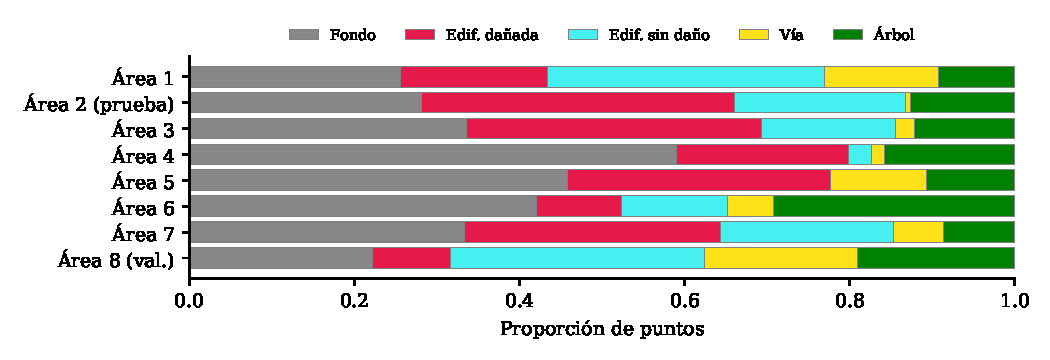
\includegraphics[width=0.8\textwidth]{figs/distribucion.pdf}
\caption{Proporción de puntos por clase en cada área tras el submuestreo. La variación entre áreas, por ejemplo la casi ausencia de vías en el Área 2, explica parte de la dificultad de generalizar entre zonas.}\label{fig:dist}
\end{figure*}

\begin{table*}[t]
\centering
\caption{Estadísticas de 3DAeroRelief calculadas por el autor. ``Puntos orig.'': puntos en los archivos originales; ``Tras vóxel'': puntos tras la alineación, la armonización de escala y el submuestreo a 0,1\,m (Sección~\ref{sec:prepro}). Las cinco últimas columnas son el porcentaje de puntos de cada clase tras el submuestreo: fondo (Fon.), edificación dañada (E.\,D.), edificación sin daño (E.\,S.), vía y árbol.}\label{tab:stats}
\footnotesize
\setlength{\tabcolsep}{4pt}
\begin{tabular}{@{}llcrrrrrrr@{}}
\toprule
Área & Uso & Nubes & \multicolumn{1}{c}{Puntos orig.\ (M)} & \multicolumn{1}{c}{Tras vóxel (M)} & Fon.\ \% & E.\,D.\ \% & E.\,S.\ \% & Vía \% & Árbol \% \\
\midrule
Área 1 & Entrenamiento & 7 & 5,7 & 2,5 & 25,6 & 17,8 & 33,6 & 13,8 & 9,2 \\
Área 2 & Prueba & 8 & 30,9 & 1,7 & 28,2 & 37,8 & 20,8 & 0,6 & 12,7 \\
Área 3 & Entrenamiento & 13 & 90,4 & 2,9 & 33,6 & 35,7 & 16,3 & 2,2 & 12,2 \\
Área 4 & Entrenamiento & 4 & 7,8 & 2,4 & 59,0 & 20,9 & 2,8 & 1,5 & 15,8 \\
Área 5 & Entrenamiento & 4 & 28,4 & 1,3 & 45,8 & 31,8 & 0,0 & 11,7 & 10,6 \\
Área 6 & Entrenamiento & 12 & 15,3 & 5,4 & 42,0 & 10,3 & 12,8 & 5,7 & 29,2 \\
Área 7 & Entrenamiento & 10 & 5,2 & 1,6 & 33,4 & 31,0 & 21,0 & 6,0 & 8,6 \\
Área 8 & Validación & 6 & 4,8 & 0,9 & 22,2 & 9,5 & 30,8 & 18,5 & 19,0 \\
\midrule
Total & --- & 64 & 188,5 & 18,8 & 37,9 & 22,2 & 16,3 & 6,4 & 17,1 \\
\bottomrule
\end{tabular}
\end{table*}

\subsection{Preprocesamiento}\label{sec:prepro}

\paragraph{Fusión de etiquetas} El color de cada punto de \texttt{segmentpp<i>.ply} se asigna a la clase cuyo color de referencia es el más cercano (distancia euclidiana en RGB). Luego, cada punto de \texttt{pp<i>.ply} recibe la etiqueta de su vecino más cercano en la nube de etiquetas, buscado con un árbol k-d. Es el mismo procedimiento del script oficial del repositorio.

\paragraph{Alineación vertical} Durante la revisión de los datos se encontró que las nubes no están alineadas con la gravedad: COLMAP entrega cada reconstrucción con una orientación arbitraria (en varias nubes, el eje ``vertical'' original es $y$). Cada nube se rota a un sistema donde $z$ es la normal del plano dominante (el eje de menor varianza según PCA, que corresponde al suelo). El sentido de $z$ se fija con las normales de superficie, que COLMAP orienta hacia la cámara y por lo tanto deben apuntar hacia arriba (hacia el dron). Las 10 nubes que no traen normales usan como regla alternativa la asimetría positiva de la distribución de alturas. Ninguna de estas reglas usa etiquetas. Como verificación a posteriori, en 62 de las 64 nubes las clases edificación y árbol quedan por encima de vía y fondo. Las dos excepciones (Área 1/pp7 sin normales y Área 3/pp11) pertenecen al conjunto de entrenamiento.

\paragraph{Armonización de escala} El artículo indica que las nubes se reescalaron con una casa de un piso de unos 3\,m como referencia~\cite{Le2026}. Sin embargo, en las Áreas 4 y 6 las edificaciones aparecen entre 3 y 3,5 veces más altas que en las demás áreas. Para cada área de entrenamiento y validación se estimó la altura típica de las edificaciones sobre el suelo (mediana de $z$ de los puntos de edificación menos el percentil 5 de $z$) y se corrigieron las áreas que se desviaban más de 1,5 veces de la mediana de las demás: factor 0,285 para el Área 4 y 0,354 para el Área 6. El Área 2 (prueba) no se usa en este cálculo ni se modifica.

\paragraph{Submuestreo por vóxel} Para homogeneizar la densidad (que varía entre capturas) y reducir el costo, se conserva un punto aleatorio por vóxel de 0,1\,m de lado. Así se pasa de 188,5 a 18,8 millones de puntos (Tabla~\ref{tab:stats}).

\paragraph{Normales de superficie} Las normales originales solo existen en 54 de las 64 nubes, así que se recalculan para todas de forma uniforme sobre los puntos submuestreados: para cada punto se toma el vector propio de menor valor propio de la covarianza de sus 16 vecinos más cercanos (PCA local) y se orienta hacia $+z$. Las normales describen la orientación local de la superficie, que cambia de forma irregular en un techo con tejas faltantes o escombros.

\paragraph{Bloques de entrada} Como una nube completa no cabe en la red, durante el entrenamiento se extraen bloques columnares de 12\,m $\times$ 12\,m en el plano XY, centrados en un punto elegido al azar. Para PointNet++ se muestrean 4096 puntos por bloque y las coordenadas se dividen por el lado del bloque, de modo que los radios de agrupación son relativos al bloque. PTv3 admite un número variable de puntos, así que recibe todos los puntos del bloque (hasta 16\,000) en coordenadas métricas.

\paragraph{Rasgos de entrada} En PointNet++ cada punto tiene 7 canales: color RGB normalizado a $[0,1]$, altura relativa dentro de la nube y posición $(x,y,z)$ normalizada respecto a la caja envolvente de la nube. En PTv3 se usan los 9 canales que esperan los codificadores preentrenados: coordenadas locales, color RGB en $[0,1]$ y normal de superficie.

\paragraph{Aumento de datos} En entrenamiento se aplican rotación aleatoria alrededor de $z$, escalado uniforme en $[0{,}9;\,1{,}1]$, reflexión en $x$, ruido gaussiano en las coordenadas ($\sigma=0{,}002$), variación de brillo y contraste, y eliminación del color con probabilidad 0,2. Esta última técnica mejora la generalización de PointNet++ según Qian et al.~\cite{Qian2022}.

\subsection{Modelos}\label{sec:modelos}

\subsubsection{PointNet++ (línea base)}

Como línea base se implementó PointNet++ en su variante de agrupación a escala única (SSG)~\cite{Qi2017b}. Se eligió por cuatro razones: (i) es la base de varios de los trabajos de daño revisados~\cite{Lou2025,Bolourian2023,Fan2024}; (ii) según PointNeXt~\cite{Qian2022}, con un entrenamiento moderno compite con arquitecturas más recientes; (iii) cabe en una GPU de consumo de 8\,GB; y (iv) no está entre los modelos evaluados en el benchmark, así que aporta un punto de comparación nuevo. La Figura~\ref{fig:arq} muestra el esquema y la Tabla~\ref{tab:capas} el detalle de las capas.

\begin{figure*}[t]
\centering
\begin{tikzpicture}[
  font=\scriptsize,
  enc/.style={draw, fill=blue!10, minimum width=13mm, align=center, rounded corners=1pt},
  dec/.style={draw, fill=orange!15, minimum width=13mm, align=center, rounded corners=1pt},
  arr/.style={-{Stealth[length=1.6mm]}},
  skip/.style={-{Stealth[length=1.6mm]}, dashed, gray}]
\node[draw, fill=gray!10, minimum height=24mm, minimum width=12mm, align=center] (in) {Entrada\\$4096\times$\\(3+7)};
\node[enc, minimum height=20mm, right=4mm of in] (sa1) {SA1\\1024\\64 c};
\node[enc, minimum height=16mm, right=3mm of sa1] (sa2) {SA2\\256\\128 c};
\node[enc, minimum height=12mm, right=3mm of sa2] (sa3) {SA3\\64\\256 c};
\node[enc, minimum height=9mm,  right=3mm of sa3] (sa4) {SA4\\16\\512 c};
\node[dec, minimum height=12mm, right=3mm of sa4] (fp4) {FP4\\64\\256 c};
\node[dec, minimum height=16mm, right=3mm of fp4] (fp3) {FP3\\256\\256 c};
\node[dec, minimum height=20mm, right=3mm of fp3] (fp2) {FP2\\1024\\128 c};
\node[dec, minimum height=24mm, right=3mm of fp2] (fp1) {FP1\\4096\\128 c};
\node[draw, fill=green!12, minimum height=24mm, minimum width=12mm, align=center, right=3mm of fp1] (head) {Cabeza\\$4096\times5$};
\foreach \a/\b in {in/sa1, sa1/sa2, sa2/sa3, sa3/sa4, sa4/fp4, fp4/fp3, fp3/fp2, fp2/fp1, fp1/head} \draw[arr] (\a) -- (\b);
\draw[skip] (sa3.north) to[out=50, in=130] (fp4.north);
\draw[skip] (sa2.north) to[out=50, in=130] (fp3.north);
\draw[skip] (sa1.north) to[out=45, in=135] (fp2.north);
\draw[skip] (in.north)  to[out=40, in=140] (fp1.north);
\node[below=2mm of sa2.south east, xshift=4mm, text width=50mm, align=center] {\textbf{Codificador}: FPS + ball query + MLP compartido + max-pool};
\node[below=2mm of fp3.south east, xshift=4mm, text width=48mm, align=center] {\textbf{Decodificador}: interpolación 3-NN + conexiones de salto};
\end{tikzpicture}
\caption{Arquitectura PointNet++ (SSG) para segmentación semántica. Bajo cada bloque se indica el número de puntos y de canales (c) de salida. Las flechas punteadas son conexiones de salto. La cabeza produce una probabilidad para cada una de las 5 clases en cada punto.}\label{fig:arq}
\end{figure*}

\begin{table}[t]
\centering
\caption{Detalle de capas de la red. $N_s$: centros muestreados por FPS; $r$: radio de agrupación (en unidades normalizadas por el lado del bloque); $K$: vecinos por grupo. Cada capa del MLP es Conv $1\times1$ + BatchNorm + ReLU.}\label{tab:capas}
\footnotesize
\begin{tabular}{@{}llccl@{}}
\toprule
Capa & Tipo & $N_s$ & $r$ / $K$ & MLP (canales) \\
\midrule
SA1 & Set abstraction & 1024 & 0,1 / 32 & $(3+7+3)\rightarrow[32,32,64]$ \\
SA2 & Set abstraction & 256 & 0,2 / 32 & $[64,64,128]$ \\
SA3 & Set abstraction & 64 & 0,4 / 32 & $[128,128,256]$ \\
SA4 & Set abstraction & 16 & 0,8 / 32 & $[256,256,512]$ \\
FP4 & Feature propagation & 64 & 3-NN & $768\rightarrow[256,256]$ \\
FP3 & Feature propagation & 256 & 3-NN & $384\rightarrow[256,256]$ \\
FP2 & Feature propagation & 1024 & 3-NN & $320\rightarrow[256,128]$ \\
FP1 & Feature propagation & 4096 & 3-NN & $135\rightarrow[128,128,128]$ \\
Cabeza & Conv $1\times1$ & 4096 & --- & $128\rightarrow128\rightarrow$ Dropout(0,5) $\rightarrow5$ \\
\midrule
\multicolumn{5}{@{}l}{Parámetros entrenables: 964\,229} \\
\bottomrule
\end{tabular}
\end{table}

Cada capa de abstracción (SA) hace tres cosas: (1) selecciona $N_s$ centros por muestreo del punto más lejano, (2) agrupa hasta $K$ vecinos dentro de un radio $r$ alrededor de cada centro y (3) aplica un MLP compartido sobre las coordenadas relativas y los rasgos de los vecinos, seguido de \emph{max pooling}. Cada capa de propagación (FP) interpola las características del nivel más escaso hacia el más denso mediante ponderación por distancia inversa de los 3 vecinos más cercanos. Además, las concatena con las características del mismo nivel del codificador (conexión de salto). Todos los operadores (FPS, \emph{ball query} e interpolación) se implementaron con operaciones tensoriales estándar de PyTorch, sin extensiones CUDA, para facilitar la instalación en Windows.

\subsubsection{Point Transformer V3 (PTv3)}

PTv3~\cite{Wu2024} reemplaza la búsqueda de vecinos por radio de PointNet++ por una \emph{serialización}: los puntos se ordenan a lo largo de curvas que recorren el espacio (curvas de Morton ``z'' y de Hilbert, y sus versiones transpuestas), y la atención se calcula dentro de parches consecutivos de 1024 puntos de esa secuencia. Así, cada punto atiende a un vecindario mucho más amplio (1024 puntos frente a los 32 de cada grupo de PointNet++), que puede abarcar una casa completa, y el costo sigue siendo bajo. Entre bloques se alterna el orden de serialización, de modo que los parches cambian de forma y la información fluye en todas las direcciones.

Se usa la implementación oficial de Pointcept, distribuida como el paquete \texttt{point-transformer-v3}. Esta versión ya no necesita las bibliotecas \texttt{spconv} ni FlashAttention y funciona en Windows con la atención estándar de PyTorch (SDPA). La Tabla~\ref{tab:ptv3} resume la configuración, que es la misma de la publicación original. La red tiene un codificador de 5 niveles (profundidades 2, 2, 2, 6 y 2; canales de 32 a 512) que reduce la resolución a la mitad entre niveles, y un decodificador de 4 niveles con conexiones de salto.

\subsubsection{PTv3 con preentrenamiento autosupervisado}

Para estudiar el efecto del preentrenamiento se parte del codificador \texttt{sonata\_small}, preentrenado con Sonata~\cite{Wu2025} sobre miles de escenas 3D sin etiquetas, y del codificador \texttt{utonia\_tiny} de Utonia~\cite{Zhang2026}, preentrenado sobre nubes de muchos dominios, incluidos escaneos aéreos. Estos codificadores no tienen decodificador. Las características de sus cinco niveles se llevan a la resolución original y se concatenan (992 canales en Sonata, 486 en Utonia), y sobre ellas se entrena una cabeza MLP ($\to256\to$ BatchNorm, ReLU, Dropout 0,3 $\to5$). Todo el modelo se ajusta (\emph{fine-tuning}): la cabeza con la tasa de aprendizaje base y el codificador con una tasa diez veces menor, para no destruir lo aprendido en el preentrenamiento.

Los codificadores preentrenados esperan una escala determinada: Sonata trabaja con celdas de 2\,cm en escenas interiores y Utonia con celdas de 1\,cm tras multiplicar las coordenadas por un factor. Por eso las coordenadas se escalan (por 0,2 en Sonata y 0,1 en Utonia) de modo que cada celda de su grilla corresponda a un vóxel de 0,1\,m del preprocesamiento, y no se pierda ningún punto.

\begin{table*}[t]
\centering
\caption{Configuración de los modelos PTv3. En todos, las profundidades del codificador son (2, 2, 2, 6, 2), la atención se calcula en parches de 1024 puntos con cuatro órdenes de serialización, y el \emph{drop path} es 0,3.}\label{tab:ptv3}
\footnotesize
\setlength{\tabcolsep}{4pt}
\begin{tabular}{@{}lccc@{}}
\toprule
 & PTv3 desde cero & Sonata (\texttt{sonata\_small}) & Utonia (\texttt{utonia\_tiny}) \\
\midrule
Pesos iniciales & Aleatorios & Preentrenados & Preentrenados \\
Canales del codificador & 32--512 & 32--512 & 18--216 \\
Decodificador & Sí (64--256) & No (concatenación) & No (concatenación) \\
Cabeza & Lineal & MLP 992--256--5 & MLP 486--256--5 \\
Celda de grilla & 0,1\,m & 0,02 (escala 0,2) & 0,01 (escala 0,1) \\
Parámetros & %%P_PTV3%% & %%P_SONATA%% & %%P_UTONIA%% \\
\bottomrule
\end{tabular}
\end{table*}

\subsection{Protocolo de entrenamiento}

Se respeta la división cruzada por áreas del benchmark~\cite{Le2026}: el Área 2 (8 nubes) es el conjunto de prueba y no se usa en ningún momento del entrenamiento ni de la selección del modelo. Como el benchmark no define un conjunto de validación, se reservó el Área 8 para seleccionar el mejor modelo, y el entrenamiento se hace con las Áreas 1, 3, 4, 5, 6 y 7. Por lo tanto, el modelo ve algo menos de datos que los modelos de referencia, una decisión conservadora que favorece a estos últimos en la comparación.

Para mitigar el desbalance de clases se usa entropía cruzada ponderada, con peso $w_c \propto 1/\sqrt{f_c}$, donde $f_c$ es la frecuencia de la clase $c$ en el entrenamiento, normalizado para que el peso medio sea 1. La Tabla~\ref{tab:hiper} resume los hiperparámetros de cada modelo. Para que la comparación sea justa, todos comparten los mismos bloques, la misma división de áreas, el mismo aumento de datos, la misma pérdida y el mismo criterio de selección del modelo (mejor mIoU en el Área 8).

\begin{table*}[t]
\centering
\caption{Hiperparámetros y entorno de entrenamiento.}\label{tab:hiper}
\footnotesize
\setlength{\tabcolsep}{4pt}
\begin{tabular}{@{}p{2.6cm}p{4.6cm}p{4.6cm}@{}}
\toprule
Parámetro & PointNet++ & PTv3 (desde cero / preentrenado) \\
\midrule
Optimizador & AdamW, \emph{weight decay} $10^{-4}$ & AdamW, \emph{weight decay} 0,05 \\
Tasa de aprendizaje & $10^{-3}$ máx. & $2\cdot10^{-3}$ máx.; codificador preentrenado: $2\cdot10^{-4}$ \\
Política & \emph{One-cycle} (calentamiento 5\,\% + coseno) & Igual \\
Lote & 16 bloques $\times$ 4096 puntos & 4 bloques completos (hasta 16\,000 puntos c/u) \\
Duración & 40 épocas $\times$ 400 iteraciones & 30 épocas $\times$ 400 iteraciones \\
Pérdida & \multicolumn{2}{l}{Entropía cruzada ponderada ($w_c \propto f_c^{-1/2}$)} \\
Precisión & Mixta (FP16) & Mixta (BF16), recorte de gradiente 10 \\
Validación & Cada 4 épocas (Área 8) & Cada 3 épocas (Área 8) \\
Semillas & \multicolumn{2}{l}{0, 1 y 2} \\
\midrule
Hardware & \multicolumn{2}{l}{GPU NVIDIA RTX 4060 Ti (8\,GB), CPU AMD Ryzen 5 5600, 32\,GB RAM} \\
Software & \multicolumn{2}{l}{Windows 11, Python 3.12, PyTorch 2.14 (CUDA 12.6), \texttt{point-transformer-v3} 0.1.2} \\
\bottomrule
\end{tabular}
\end{table*}

\subsection{Protocolo de evaluación}

La inferencia se hace sobre cada nube completa del Área 2 con una ventana deslizante de 12\,m $\times$ 12\,m y paso igual a la mitad del lado. Todos los puntos de cada ventana se procesan en grupos de 4096. Como las ventanas se solapan, cada punto recibe varias predicciones; se suman las probabilidades y se toma la clase de mayor probabilidad acumulada. Con la matriz de confusión acumulada sobre todo el conjunto de prueba se calculan:
\begin{align}
\mathrm{IoU}_c &= \frac{TP_c}{TP_c+FP_c+FN_c}, & \mathrm{mIoU} &= \frac{1}{C}\sum_{c=1}^{C}\mathrm{IoU}_c, \\
\mathrm{Acc}_c &= \frac{TP_c}{TP_c+FN_c}, & \mathrm{mAcc} &= \frac{1}{C}\sum_{c=1}^{C}\mathrm{Acc}_c, \\
F1_c &= \frac{2\,TP_c}{2\,TP_c+FP_c+FN_c}, & \mathrm{OA} &= \frac{\sum_c TP_c}{N},
\end{align}
donde $C=5$ es el número de clases y $N$ el número de puntos evaluados. mIoU y mAcc se definen igual que en el benchmark~\cite{Le2026}, de modo que los resultados son directamente comparables.

\paragraph{Resolución original} Los modelos predicen sobre los puntos submuestreados a 0,1\,m. Para reportar el desempeño sobre la nube completa (30,9 millones de puntos en el Área 2), cada punto original recibe la predicción de su vecino submuestreado más cercano, aplicando antes la misma alineación vertical del preprocesamiento.

\paragraph{Aumento en prueba (TTA)} Opcionalmente, cada nube se predice ocho veces (cuatro rotaciones de $90^\circ$ alrededor de $z$, con y sin reflexión) y se promedian las probabilidades.

\paragraph{Semillas} Según el presupuesto de cómputo, cada configuración se entrenó con hasta tres semillas (0, 1 y 2), priorizando los modelos preentrenados; el número exacto se indica en la Tabla~\ref{tab:final}. Se reporta la media $\pm$ la desviación estándar, para distinguir diferencias reales de variaciones aleatorias del entrenamiento.

\subsection{Implementación, reproducibilidad y herramienta}\label{sec:impl}

El proyecto se organizó como un producto de software reproducible. El repositorio público (\url{https://github.com/Jhodave31/deteccion-danos-nubes-puntos}) contiene: los módulos de preprocesamiento, modelos, entrenamiento y evaluación (\texttt{code/}); un guion que ejecuta todos los experimentos en cadena (\texttt{run\_all.sh}); tres notebooks ejecutados con sus salidas (\texttt{notebooks/}: datos y preprocesamiento, modelos y entrenamiento, y evaluación); las métricas de cada corrida (\texttt{runs/}); y, como \emph{release}, los modelos entrenados. El notebook de evaluación vuelve a ejecutar un modelo entrenado sobre el área de prueba y reproduce las métricas reportadas; todas las tablas y figuras de la Sección~\ref{sec:resultados} se generan con el mismo código (\texttt{aggregate.py}) a partir de esas métricas.

Además, el modelo se integró en una aplicación web local para que un usuario sin conocimientos de aprendizaje profundo pueda analizar una nube. Sus requisitos funcionales son: seleccionar una nube del dataset o cargar un \texttt{.ply} propio, segmentarla con el mismo preprocesamiento del experimento, visualizarla en 3D (coloreada por predicción, color real, etiqueta real o mapa de errores) y resumir la proporción de cada clase. Sus requisitos no funcionales son funcionar sin conexión, responder en segundos y no requerir instalación adicional. La arquitectura es cliente-servidor local (Figura~\ref{fig:arqsw}): un servidor en Python (biblioteca estándar \texttt{http.server}) \emph{reutiliza} los módulos del experimento mediante una clase \texttt{Predictor}, que carga cualquiera de los modelos entrenados a partir de su carpeta de resultados; el cliente es una página web con \texttt{three.js}, incluida localmente, que dibuja hasta 700\,000 puntos de forma interactiva.

\begin{figure}[t]
\centering
\begin{tikzpicture}[
  node distance=4mm and 3mm,
  box/.style={draw, rounded corners=2pt, align=center, font=\scriptsize, minimum height=10mm, text width=19mm, fill=#1},
  box/.default=gray!8,
  arr/.style={-{Stealth[length=2mm]}, thick}]
\node[box=blue!8] (ui) {\textbf{Navegador}\\interfaz web\\+ visor \texttt{three.js}};
\node[box=orange!12, right=9mm of ui] (srv) {\textbf{Servidor local}\\\texttt{app.py}\\(\texttt{http.server})};
\node[box, right=of srv, yshift=8mm] (pre) {Preprocesamiento\\\texttt{preprocess.py}\\\texttt{add\_normals.py}};
\node[box=green!10, right=of srv, yshift=-8mm] (pred) {\texttt{Predictor}\\PointNet++ / PTv3\\(PyTorch, GPU)};
\node[box, below=of srv] (data) {Dataset y modelos\\\texttt{data/}, \texttt{runs/}};
\draw[arr, <->] (ui) -- node[below, font=\tiny] {HTTP} (srv);
\draw[arr] (srv) -- (pre); \draw[arr] (srv) -- (pred); \draw[arr, <-] (srv) -- (data);
\end{tikzpicture}
\caption{Arquitectura de la herramienta. Todo se ejecuta en el computador del usuario, sin servicios externos.}\label{fig:arqsw}
\end{figure}

%% ====================================================================
\section{Resultados}\label{sec:resultados}

%%RESULTS%%

\subsection{Herramienta en funcionamiento}\label{sec:herramienta}

\begin{figure*}[t]
\centering
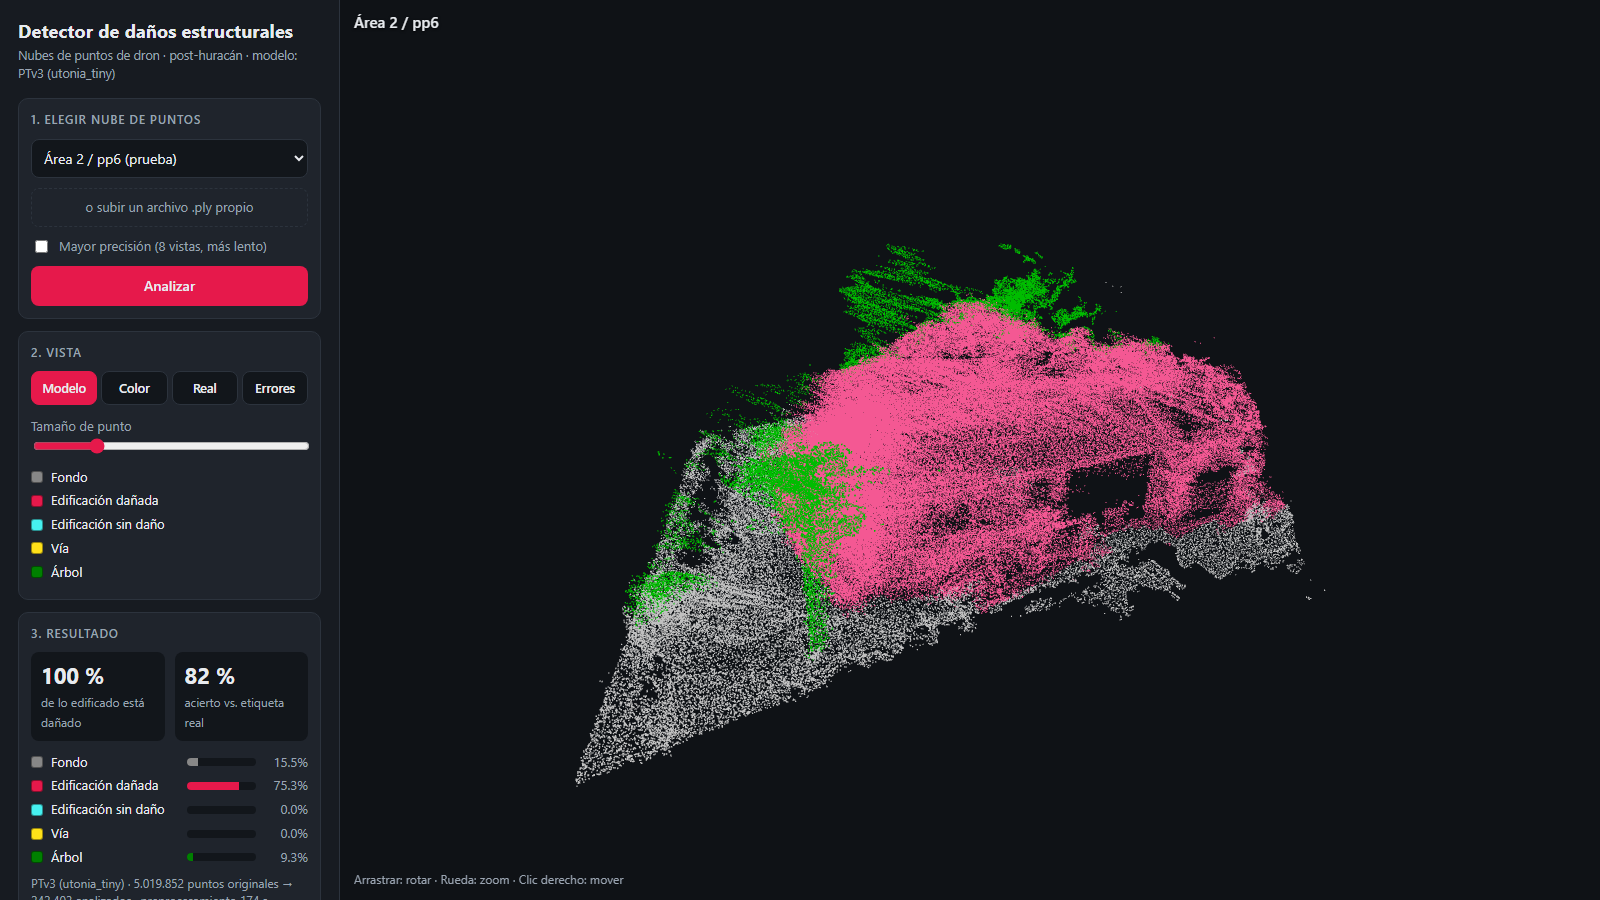
\includegraphics[width=0.82\textwidth]{figs/demo.png}
\caption{Interfaz de la herramienta analizando una nube de prueba (Área 2). A la izquierda, la selección de la nube, los modos de vista y el resumen; a la derecha, el visor 3D con la predicción del modelo: edificación dañada (rojo), edificación sin daño (celeste), vegetación (verde), vías (amarillo) y fondo (gris).}\label{fig:demo}
\end{figure*}

La Figura~\ref{fig:demo} muestra la herramienta analizando una nube de prueba con el modelo PTv3 + Utonia. %%SOFTWARE_PERF%% Se verificó que reproduce las predicciones de la evaluación (el acierto mostrado coincide con el del guion de evaluación sobre los mismos puntos), y se probaron los cuatro modos de vista, la carga de archivos propios y la ejecución sin conexión.

%% ====================================================================
\section{Discusión}\label{sec:discusion}

%%DISCUSSION%%


%% ====================================================================
\section{Conclusiones y trabajo futuro}\label{sec:conclusiones}

%%CONCLUSIONS%%

%% ====================================================================
%% ====================================================================
\begin{thebibliography}{99}

\bibitem{Hake2023} F.~Hake, P.~Lippmann, H.~Alkhatib, V.~Oettel, I.~Neumann, Automated damage detection for port structures using machine learning algorithms in heightfields, Applied Geomatics 15(2) (2023) 349--357. \url{https://doi.org/10.1007/s12518-023-00493-z}

\bibitem{Chen2025} S.~Chen, G.~Fan, J.~Li, H.~Hao, Automatic complex concrete crack detection and quantification based on point clouds and deep learning, Engineering Structures 327 (2025) 119635. \url{https://doi.org/10.1016/j.engstruct.2025.119635}

\bibitem{Chen2021} X.~Chen, J.~Li, S.~Huang, H.~Cui, P.~Liu, Q.~Sun, An automatic concrete crack-detection method fusing point clouds and images based on improved Otsu's algorithm, Sensors 21(5) (2021) 1581. \url{https://doi.org/10.3390/s21051581}

\bibitem{Dorafshan2018} S.~Dorafshan, R.~J. Thomas, M.~Maguire, SDNET2018: An annotated image dataset for non-contact concrete crack detection using deep convolutional neural networks, Data in Brief 21 (2018) 1664--1668. \url{https://doi.org/10.1016/j.dib.2018.11.015}

\bibitem{Lou2025} Y.~Lou, S.~Meng, Y.~Zhou, Deep learning-based three-dimensional crack damage detection method using point clouds without color information, Structural Health Monitoring 24(2) (2025) 657--675. \url{https://doi.org/10.1177/14759217241236929}

\bibitem{Le2026} N.~Le, E.~Karimi, M.~Rahnemoonfar, 3DAeroRelief: The first 3D benchmark UAV dataset for post-disaster assessment, Scientific Data 13 (2026) 1305. \url{https://doi.org/10.1038/s41597-026-07341-w}

\bibitem{Zahs2023} V.~Zahs, K.~Anders, J.~Kohns, A.~Stark, B.~Höfle, Classification of structural building damage grades from multi-temporal photogrammetric point clouds using a machine learning model trained on virtual laser scanning data, International Journal of Applied Earth Observation and Geoinformation 122 (2023) 103406. \url{https://doi.org/10.1016/j.jag.2023.103406}

\bibitem{Jing2024} Y.~Jing, J.-X. Zhong, B.~Sheil, S.~Acikgoz, Anomaly detection of cracks in synthetic masonry arch bridge point clouds using fast point feature histograms and PatchCore, Automation in Construction 168 (2024) 105766. \url{https://doi.org/10.1016/j.autcon.2024.105766}

\bibitem{Jing2025} Y.~Jing, W.~Lin, B.~Sheil, S.~Acikgoz, 3D multimodal feature for infrastructure anomaly detection, Automation in Construction 178 (2025) 106388. \url{https://doi.org/10.1016/j.autcon.2025.106388}

\bibitem{Dais2021} D.~Dais, I.~E. Bal, E.~Smyrou, V.~Sarhosis, Automatic crack classification and segmentation on masonry surfaces using convolutional neural networks and transfer learning, Automation in Construction 125 (2021) 103606. \url{https://doi.org/10.1016/j.autcon.2021.103606}

\bibitem{Jing2022} Y.~Jing, B.~Sheil, S.~Acikgoz, Segmentation of large-scale masonry arch bridge point clouds with a synthetic simulator and the BridgeNet neural network, Automation in Construction 142 (2022) 104459. \url{https://doi.org/10.1016/j.autcon.2022.104459}

\bibitem{SanchezAparicio2025} L.~J. Sánchez-Aparicio, R.~Santamaría-Maestro, P.~Sanz-Honrado, P.~Villanueva-Llauradó, et~al., A holistic solution for supporting the diagnosis of historic constructions from 3D point clouds, Remote Sensing 17(12) (2025) 2018. \url{https://doi.org/10.3390/rs17122018}

\bibitem{SanzHonrado2026} P.~Sanz-Honrado, R.~Santamaría-Maestro, L.~J. Sánchez-Aparicio, Seg4D: An open-source solution for supporting the diagnosis of historic constructions using 3D point clouds -- A case study application, The International Archives of the Photogrammetry, Remote Sensing and Spatial Information Sciences XLVIII-2/W12-2026 (2026) 439--446. \url{https://doi.org/10.5194/isprs-archives-XLVIII-2-W12-2026-439-2026}

\bibitem{Loverdos2024} D.~Loverdos, V.~Sarhosis, Pixel-level block classification and crack detection from 3D reconstruction models of masonry structures using convolutional neural networks, Engineering Structures 310 (2024) 118113. \url{https://doi.org/10.1016/j.engstruct.2024.118113}

\bibitem{Ye2024} Z.~Ye, L.~Lovell, A.~Faramarzi, J.~Nini\'{c}, SAM-based instance segmentation models for the automation of structural damage detection, Advanced Engineering Informatics 62 (2024) 102826. \url{https://doi.org/10.1016/j.aei.2024.102826}

%% ---- Referencias nuevas (segunda entrega) ----

\bibitem{Qi2017a} C.~R. Qi, H.~Su, K.~Mo, L.~J. Guibas, PointNet: Deep learning on point sets for 3D classification and segmentation, in: Proceedings of the IEEE Conference on Computer Vision and Pattern Recognition (CVPR), 2017, pp. 77--85. \url{https://doi.org/10.1109/CVPR.2017.16}

\bibitem{Qi2017b} C.~R. Qi, L.~Yi, H.~Su, L.~J. Guibas, PointNet++: Deep hierarchical feature learning on point sets in a metric space, in: Advances in Neural Information Processing Systems 30 (NeurIPS), 2017, pp. 5099--5108. \url{https://arxiv.org/abs/1706.02413}

\bibitem{Qian2022} G.~Qian, Y.~Li, H.~Peng, J.~Mai, H.~A. A.~K. Hammoud, M.~Elhoseiny, B.~Ghanem, PointNeXt: Revisiting PointNet++ with improved training and scaling strategies, in: Advances in Neural Information Processing Systems 35 (NeurIPS), 2022, pp. 23192--23204. \url{https://doi.org/10.52202/068431-1685}

\bibitem{Zhao2021} H.~Zhao, L.~Jiang, J.~Jia, P.~Torr, V.~Koltun, Point Transformer, in: Proceedings of the IEEE/CVF International Conference on Computer Vision (ICCV), 2021, pp. 16239--16248. \url{https://doi.org/10.1109/ICCV48922.2021.01595}

\bibitem{Wu2022} X.~Wu, Y.~Lao, L.~Jiang, X.~Liu, H.~Zhao, Point Transformer V2: Grouped vector attention and partition-based pooling, in: Advances in Neural Information Processing Systems 35 (NeurIPS), 2022, pp. 33330--33342. \url{https://doi.org/10.52202/068431-2415}

\bibitem{Wu2024} X.~Wu, L.~Jiang, P.-S. Wang, Z.~Liu, X.~Liu, Y.~Qiao, W.~Ouyang, T.~He, H.~Zhao, Point Transformer V3: Simpler, faster, stronger, in: Proceedings of the IEEE/CVF Conference on Computer Vision and Pattern Recognition (CVPR), 2024, pp. 4840--4851. \url{https://doi.org/10.1109/CVPR52733.2024.00463}

\bibitem{Peng2024} B.~Peng, X.~Wu, L.~Jiang, Y.~Chen, H.~Zhao, Z.~Tian, J.~Jia, OA-CNNs: Omni-adaptive sparse CNNs for 3D semantic segmentation, in: Proceedings of the IEEE/CVF Conference on Computer Vision and Pattern Recognition (CVPR), 2024, pp. 21305--21315. \url{https://doi.org/10.1109/CVPR52733.2024.02013}

\bibitem{Park2022} C.~Park, Y.~Jeong, M.~Cho, J.~Park, Fast Point Transformer, in: Proceedings of the IEEE/CVF Conference on Computer Vision and Pattern Recognition (CVPR), 2022, pp. 16928--16937. \url{https://doi.org/10.1109/CVPR52688.2022.01644}

\bibitem{Rahnemoonfar2023} M.~Rahnemoonfar, T.~Chowdhury, R.~Murphy, RescueNet: A high resolution UAV semantic segmentation dataset for natural disaster damage assessment, Scientific Data 10 (2023) 913. \url{https://doi.org/10.1038/s41597-023-02799-4}

\bibitem{Hu2022} Q.~Hu, B.~Yang, S.~Khalid, W.~Xiao, N.~Trigoni, A.~Markham, SensatUrban: Learning semantics from urban-scale photogrammetric point clouds, International Journal of Computer Vision 130(2) (2022) 316--343. \url{https://doi.org/10.1007/s11263-021-01554-9}

\bibitem{Bolourian2023} N.~Bolourian, M.~Nasrollahi, F.~Bahreini, A.~Hammad, Point cloud-based concrete surface defect semantic segmentation, Journal of Computing in Civil Engineering 37(2) (2023) 04022056. \url{https://doi.org/10.1061/JCCEE5.CPENG-5009}

\bibitem{Fan2024} J.~Fan, W.~Song, J.~Zhang, S.~Sun, G.~Jia, G.~Jin, PAN: Improved PointNet++ for pavement crack information extraction, Electronics 13(16) (2024) 3340. \url{https://doi.org/10.3390/electronics13163340}

\bibitem{Liu2025} S.~Liu, K.~Isobe, J.~Si, D.~Li, D.~Ren, A multi-module deep learning framework with graph-based network and crack attention for tunnel lining crack segmentation from LiDAR point cloud, Construction and Building Materials 494 (2025) 143383. \url{https://doi.org/10.1016/j.conbuildmat.2025.143383}

\bibitem{Xu2025} H.~Xu, M.~Wang, C.~Liu, Y.~Guo, Z.~Gao, C.~Xie, Tunnel crack assessment using simultaneous localization and mapping (SLAM) and deep learning segmentation, Automation in Construction 171 (2025) 105977. \url{https://doi.org/10.1016/j.autcon.2025.105977}

\bibitem{Yang2023} X.~Yang, E.~del Rey Castillo, Y.~Zou, L.~Wotherspoon, Semantic segmentation of bridge point clouds with a synthetic data augmentation strategy and graph-structured deep metric learning, Automation in Construction 150 (2023) 104838. \url{https://doi.org/10.1016/j.autcon.2023.104838}

\bibitem{Shah2025} S.~Shah, J.~Shan, P.~Li, UAV-based 3D segmentation and structural damage assessment of regional buildings, Journal of Civil Structural Health Monitoring 15(8) (2025) 4081--4105. \url{https://doi.org/10.1007/s13349-025-01030-9}

%% ---- Referencias nuevas (entrega final) ----

\bibitem{Wu2025} X.~Wu, D.~DeTone, D.~Frost, T.~Shen, C.~Xie, N.~Yang, J.~Engel, R.~Newcombe, H.~Zhao, J.~Straub, Sonata: Self-supervised learning of reliable point representations, in: Proceedings of the IEEE/CVF Conference on Computer Vision and Pattern Recognition (CVPR), 2025, pp. 22193--22204. \url{https://doi.org/10.1109/CVPR52734.2025.02067}

\bibitem{Zhang2026} Y.~Zhang, X.~Wu, Y.~Yang, X.~Fan, H.~Li, Y.~Zhang, Z.~Huang, N.~Wang, H.~Zhao, Utonia: Toward one encoder for all point clouds, in: International Conference on Machine Learning (ICML), 2026. \url{https://arxiv.org/abs/2603.03283}

\end{thebibliography}

\end{document}
